%%%%%%%%%%%%%%%%%%%%%%%%%%%%%%%%%%%%%%%%%%%%%%%%%%%%%%%%%%%%%%%%%%%%%%%%%%%%%%%%
%% Sample document ``thesis.tex''
%%

% Available documentclass options:
% - <all `report` document class options, e.g.: `a5paper`>
\documentclass[]{simple-thesis}


%%%%%%%%%%%%%%%%%%%%%%%%%%%%%%%%%%%%%%%%%%%%%%%%%%%%%%%%%%%%%%%%%%%%%%%%%%%%%%%%
%% Some mods
%%
\usepackage{graphicx}
\usepackage{courier}
\usepackage{listings}
\usepackage[margin=1cm]{caption}
\usepackage[toc]{appendix}
\usepackage{array}
\usepackage{float}
\usepackage{csquotes}
\newcolumntype{C}{>{\centering\arraybackslash}p{1.5cm}}
\renewcommand{\labelitemii}{$\circ$}  % Set the nested itemize style to empty circle.
\lstset{
  basicstyle=\footnotesize\ttfamily,
  numbers=left
}
\newcommand\fnurl[2]{%
  \href{#2}{#1}\footnote{\url{#2}}%
}


%%%%%%%%%%%%%%%%%%%%%%%%%%%%%%%%%%%%%%%%%%%%%%%%%%%%%%%%%%%%%%%%%%%%%%%%%%%%%%%%
%% Thesis meta-information
%%

%% The title of the thesis:
\title{UnsocialVR: Faking active listening in social virtual environments}

%% The full name of the author (e.g.: James Smith):
\author{Tom Gurion}

%% Affiliation:
\affiliation{Media and Arts Technology\\Queen Mary University of London}
\affiliationlogo{CollegeShields/QMUL}

%% You can redefine the submission notice [optional]:
\submissionnotice{Advanced placement project final report\\Supervisor: Patrick Healey\\Host: Inition}

%% PDF meta-info:
\hypersetup{pdfsubject={TODO subject},pdfkeywords={TODO keywords}}


%%%%%%%%%%%%%%%%%%%%%%%%%%%%%%%%%%%%%%%%%%%%%%%%%%%%%%%%%%%%%%%%%%%%%%%%%%%%%%%%
%% Abstract:
%%
\abstract{%
  TODO abstract...
}


%%%%%%%%%%%%%%%%%%%%%%%%%%%%%%%%%%%%%%%%%%%%%%%%%%%%%%%%%%%%%%%%%%%%%%%%%%%%%%%%
%% Acknowledgements:
%%
\acknowledgements{%
  TODO acknowledgments...

  Patrick Healey.
  Inition.
  Pedro.
  Stuart.
}


%%%%%%%%%%%%%%%%%%%%%%%%%%%%%%%%%%%%%%%%%%%%%%%%%%%%%%%%%%%%%%%%%%%%%%%%%%%%%%%%
%% Contents:
%%
\begin{document}

\frontmatter{}  %% Title page, abstract, TOC, etc.


%%%%%%%%%%%%%%%%%%%%%%%%%%%%%%%%%%%%%%%%%%%%%%%%%%%%%%%%%%%%%%%%%%%%%%%%%%%%%%%%
%% Thesis body:
%%
\setcounter{page}{1}  % Start page count from here
\chapter{Introduction}

In Infinite Jest, David Foster Wallace argues that ``Good old traditional audio-only phone conversations allowed you to presume that the person on the other end was paying complete attention to you while also permitting you not to have to pay anything even close to complete attention to her.'' \citep{Wallace1996}.
He continues and claims that we are addicted to this illusion, and that's why video conferencing always feel so awkward - we need to pretend to listen all the time.
And if we think about it, even in face to face conversation we must always adhere to these social rules, and signal our complete attention when someone is talking to us.

In this project I experiment with virtual reality (VR) technologies to see if this illusion of faking active listening is transferable to other mediums, and if so, how.
In Unsocial VR participants share the same virtual environment, using VR headsets and controllers.
They can converse freely and move around, and if they want to start faking listening to the conversation and just wander around, or even talk with other participants while faking, they absolutely can!
The interface is very minimal, just hit a button on the controller to start faking active listening behaviours towards your current conversation, and release it when you want to stop faking.
Players even get an on screen notification when someone is speaking directly to them, so they can return to the conversation elegantly.

TODO More generally...
Social VR as an environment to investigate behaviours.

Chapter \ref{literature_review} review the relevant literature on the topics relevant for the current study.
Chapter \ref{system_design_and_implementation} present the system developed for the study, including detailed motivation for each decision.
Chapter \ref{evaluation} show the evaluation of the system.
Chapter \ref{general_discussion} discuss the finding.
Chapter \ref{conclusions} conclude this report with TODO and suggestions for future work.


\chapter{Literature review}\label{literature_review}

TODO rewrite.
This project is based on multidisciplinary research.
It merges ideas from telepresence and mediated communication, that explore the representation of non verbal cues in new communication technologies;
depends on multiparty social interaction analysis, which uses spatial cues to understand who is talking with whom in dynamic social environments;
make use of new ways to generate active listening cues, such as head nods, in automated agents;
and influenced by research in asymmetric social communication in virtual environments.

\section{Collaborative virtual environments}

Collaborative virtual environments (CVEs) are computer systems that generate 3D avatars to represent human participants in a shared virtual space \citep{Bailenson2004}.
Recent technological breakthroughs made CVEs a possible advancement for both telecommunication and social research.
This section presents the advantages of using CVEs for both use cases.

Telecommunication technologies often tries to maximize the feeling of being together at a remote location.
This feeling, known as \textit{social presence}, varies between different communication media \citep{Short1976}.
For example, video conferencing is often described as a medium that supports higher social presence than, let's say, text-only chats.
But video conferencing is still way behind face-to-face conversation in many senses.
In multiparty conversation, its shortcomings include decreased turn taking efficiency, inability to participate in side conversations, lack of meaningful gaze, and no 3 dimensional orientation \citep{Isaacs1994}.

CVEs attempt to solve some of these issues by exposing socially significant cues in the virtual environment.
One of these cues, that is not redundantly coded in speech, and is usually problematic in video conferencing, is gaze.
CVEs that convey gaze give clear indication of who is talking with whom, and therefore simplify the turn taking management \citep{Vertegaal1999, Vertegaal2003}.
In addition, researchers show that exposing the participants eye gaze in the virtual environment improved their lying detection \citep{Steptoe2010}.
Other studies explore the effects of non-verbal cues on communication.
For example, participants in CVEs that track and render head movements reported higher social presence compared to environments with static, non-moving, heads.
Participants in the first condition also reported that they liked each other more, and looked more on the other participant head \citep{Bailenson2002}.
Similarly, when trying to communicate the meaning of a word, participants performed better when their listener's hand movements were presented in the virtual environment \citep{Dodds2011}.

Recently, the interest in CVEs started to spread beyond the research community.
Social VR attempts to bring CVEs to social media users with tight integration with existing and new social media platforms \citep{Bonasio2016}.
It is of no surprise that reviews of these commercial products tend to highlight known CVEs advantages compared to other ways of communication.
Namely, the possibility to create eye contact, the use of body language, free movement, higher social presence, and more \citep{Rosedale2015}.
Eye tracking is not yet supported by any social VR product.
The reason is probably the lack of available consumer VR headsets with eye tracking.
Regardless, introducing eye tracking to social VR seems to be a natural step forwards \citep{Langley2017}.
Yet again, the lessons learned from research in non verbal cues in CVEs are inline with the market demands.

The use of CVEs is not bounded to telecommunication.
They are also a great tool for social research.
Traditionally, controlled experiments often explore psychological and social concepts out of context, in a laboratory environment.
Consequently, the ecological validity of the results might be unclear.
VR provides a possible solution to this issue, by providing a controlled environment that preserves the context and therefore increase the results' ecological validity \citep{Loomis1999}.
Researchers also suggest that VR might solve two more common issues in psychology: the lack of replications, and unrepresentative sampling.
First, the field suffer from lack of replications.
When the entire experiment is done in VR, instead of complex laboratory setup, replication might be easier.
Second, participants in experiments are often not a representative sample.
As already discussed, VR is becoming more widespread and with the emergence of social VR more users interact daily with VR content.
In the future, VR might help mitigating the unrepresentative sampling issue by allowing scientist to run experiments with remote participants.
With the right consumer technology, it is not impossible that participation in immersive social experiments will become as simple as filling an online survey \citep{Blascovich2002}.

\section{Transformed social interaction}

Transformed social interaction \citep{Bailenson2004, Bailenson2008}.

Asymmetric communication \citep{Chou2016, Yee2007, Dominguez2014}.

\section{Active listening and embodied conversational agents}

In order to make a conversation natural and engaging, conversing parties transmit a wide array of social cues.
These signals can indicate the parties interest in keeping the conversation going, show mutual understanding, or the attempt to take the speaker turn.
Whereas conversations are usually considered to be a lingual phenomena, many of these social signals are non-verbal (e.g.\ head nods and facial expressions), or paralingual (e.g.\ the use of prosody or utterances like ``uh-huh'').
In the context of active listening behaviours these are known as backchannels, and there are reasons to believe that they can be modeled without attending the content of the conversation \citep{Yngve1970}.
Backchannel behaviours are known to have a significant effect on the speaker \citep{Bavelas2000} and are important for establishing rapport \citep{Gratch2007}.
Therefore, it is of no surprise that one of the main application for backchannels research is the automation of embodied conversational agents (ECAs).
Integrating backchannels into such agents might be the key to providing socially appropriate responses in free conversation \citep{Morency2008, Bevacqua2008}.

Researchers often use surface features like speaker-listener eye contact, speaker voice level, and prosody to model backchannels.
\citeauthor{Ward2000} suggested a backchannel prediction model that is based on the speaker prosody (\citeyear{Ward2000}).
Their model uses a small set of features and simple hand-crafted rules.
Specifically, speaker ``talking state'' (speaking or silent) and the pitch of the speaker voice were taken into account.
\citeauthor{Gratch2006} propose to incorporate the speaker head moves and body pose into a similar model (\citeyear{Gratch2006}).
\citeauthor{Lee2006}, on the other hand, suggested to use surface text features to predict backchannels (\citeyear{Lee2006}).
They used a bag-of-words technique, with different spoken words triggering different listener responses.
They based their rules on manual analysis of recorded video conversations with ECAs.
All of these studies use a set of carefully chosen hand-crafted rules to build their backchannel prediction models.

Recent studies suggest data-driven approaches for backchannels modeling to improve predictive performance.
\citeauthor{Nishimura2007} predict listener responses using the pitch and power of the speaker voice (\citeyear{Nishimura2007}).
Their model, however, isn't constrained to predict backchannels only.
A response generator uses audio features to choose between types of responses, like backchannels, collaborative completion (e.g. suggesting a keyword for the speaker), and more.
Their decision-tree model was trained using audio-recorded and annotated conversations of the RWC multimodal database \citep{Hayamizu1996}.
\citeauthor{Morency2008} followed a similar path but with a more exhaustive set of audio-based features, and speaker-listener gaze annotations (\citeyear{Morency2008}).
In addition, they encoded each feature with a set of encoding templates that modified the appearance of the feature over time.
Then, they applied probabilistic methods to choose the feature with the most predictive power to incorporate into the model.
\citeauthor{Huang2011} uses a simplified model that is based only on non-verbal information (\citeyear{Huang2011}).
Their model uses the speaker talking state, speaker-listener eye contact, and, interestingly, the speaker smile, to predict listener backchannels.
A year later, \citeauthor{Kok2012} suggested some improvements to the same model to make it more robust to different speaker behaviours (\citeyear{Kok2012}).
Note that there is almost no direct comparison between the different models, mainly due to the use of different datasets and different evaluation methods \citep{Morency2008}.

Before ending this section, it is important to discuss the theoretical differences between conversing parties in a social interaction.
Some of the roles in a conversation are more obvious, like the role of the speaker.
The differences between other roles, however, might be harder to tell.
According to \citeauthor{Clark1982}, apart from the speaker, participants in a conversation can take a role of addressees, side-participants, and over-hearers (\citeyear{Clark1982}).
Put simply, addressees are the listeners that the speaker illocutionary act is directed to.
Side-participants are the listeners that the speaker wish to inform about his/her illocutionary act towards the addressees.
Although they usually not expected to take the floor, they are an important part of the conversation.
The speaker must take the side-participants understanding in mind, and expected them to confirm their understanding, probably through non verbal cues (TODO find ref).
Over-hearers are listeners that the speaker have no interest in them hearing the conversation.
They are less relevant for the current study and thus won't be further discussed.
The roles are usually assigned to the participants, implicitly, by the speaker.

Most of the current research in backchannels and active listening behaviour is concentrated on two party conversations.
Therefore, side-participants active listening behaviours are much less investigated, understood, and modeled.
TODO present \citep{Matsusaka2003, Fujie2009}.


\chapter{System design and implementation}\label{system_design_and_implementation}

Whereas many studies explore active listening behaviours using ECAs \citep{Nishimura2007, Bevacqua2008, Gratch2007, Huang2011, Lee2006, Poppe2013}, the current research aim to investigate how humans can start to pretend to listen to someone, how they stop faking and return to the conversation, and what are the social implication for such behaviours.
Recently, social research see high opportunities in exploring social behaviours using virtual environments \citep{Bailenson2008}.
Following the same trend, and inspired by the possibilities to fake attention in ways that are impossible in face-to-face conversation, the current research is based on a social virtual environment system.

The main target of the system is to support exploration of faked active listening behaviours in a multiparty social context.
As such, it implements a shared virtual environment, and uses a minimal user interface to let participants start and stop faking.
Using this interface users can press a button to start faking, meaning, that while the button is pressed other users won't see the real behaviour of this user in the virtual environment.
Instead, the avatar of the faking user, as viewed by the other users, will be controlled by an automated behaviour.
The three principles that enable this automation are presented in section \ref{system:mechanisms}.
In the background, a set of software components analyze the social interaction and manipulate how each participant experience the environment.

Figure \ref{fig:system:diagram} shows a schematic diagram of the system architecture, and the paths and protocols of communication between the components.
In blue are the client side components.
The components in green are client facing servers, and the red ones are background servers that process behavioural data to instruct the client facing servers how to operate.
A thorough description of each component in the system is presented bellow.

The code-base for the entire project is open sourced and \fnurl{available online}{https://github.com/Nagasaki45/UnsocialVR}.

\begin{figure}
  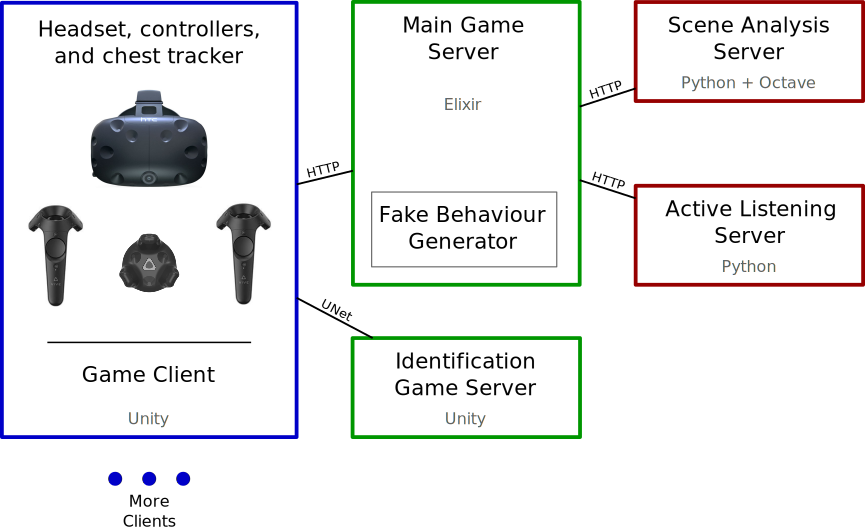
\includegraphics[width=\textwidth]{../graphics/system_diagram.pdf}
  \caption{A schematic diagram of the system architecture. In blue are client side components, that communicate with the client facing servers in green. The components in red are background servers that are used by the client facing servers to process behavioural data. The lines between the components represents paths of communication with the a label indicating the protocol.}
  \label{fig:system:diagram}
\end{figure}

\section{Mechanisms for faking active listening behaviour}\label{system:mechanisms}

The underlying mechanisms that support the automation of the faking behaviour are a mixture of ideas.
Part of them are based on the scientific literature, while others are novel findings from the current research.

\subsection{Automated head nods}

As already discussed, carefully crafted automated head nods are known to be crucial for creating convincing ECAs.
Therefore, the current project follows the literature in the field and implements a machine learning based backchannel predictor.
This predictor is thoroughly described in section \ref{system:active_listening_server}.

\subsection{Baseline recorded movement}

When users trigger the automated behaviour their avatars must keep moving naturally.
They can't, for example, just freeze.
During the early development phases of the system the faked behaviour used a pre-recorded movement of the hands, head, and chest.
This pre-recorded movement was looped to support an arbitrary length of faking periods.
In addition, random time lag was added for the recorded movement of each user to make sure no two fakers look the same.

At that time, I ran an unofficial pilot study with 3 co-workers to expose user experience issues with the system.
Participants in the pilot were not instructed to do any specific task in the virtual environment, nor fill any questionnaire before or after the experience.
In addition, no measurements were recorded.
Instead, I was interested to hear from the participants about their experience with the system, and probed them to emphasis their experience with the faking mechanism.

The results clearly show that the transitions into automated behaviour are noticeable.
The change of body posture and the positioning change of the body parts between the real and the faked behaviour were easily detected.
The reason for that is that physical differences between people are recreated in the virtual environment.
Ignoring these and using the same movement for everyone allowed the participants to quickly learn to notice the pre-recorded behaviour.

The solution I found is to always record the last few seconds of each user.
When the user trigger the faked behaviour this recorded movement will start to play in a loop.
To make sure that there is no jump in the loop the recorded movement is first played backwards from the last recorded sample.
Whenever the playing head reaches the end of the recorded movement the playing direction flips.
More implementation details are described in section \ref{system:fake_behaviour_generator}.

\subsection{Looking at the speaker}

With the head nods and the baseline recorded movement in place there was a need for modeling the avatar attention in one way or another.
A basic approximation of attention in a conversation is to always look at the speaker.
Therefore, the last underlying mechanism for the faked behaviour is to always slowly rotate towards the user that is speaking.
If no one is speaking, I choose to rotate the faking avatars towards the last speaker.

\section{Hardware}

The hardware used in this project is the \fnurl{HTC Vive}{https://www.vive.com/uk/}, which bundle together a headset and two hand controllers.
In addition, a \fnurl{Vive tracker}{https://www.vive.com/uk/vive-tracker/} is used to track the chest position of each participant.
This setup provided suitable features for the project compared to products like the \fnurl{Oculus Rift}{https://www.oculus.com/rift/}, or simpler VR solutions like \fnurl{Google Daydream}{https://vr.google.com/daydream/} or \fnurl{Samsung Gear VR}{http://www.samsung.com/global/galaxy/gear-vr/}.
Specifically, my system make use of the following features of the headset, that I couldn't find in other products:

\begin{itemize}
  \item The headset and its controllers and trackers are tracked in 3 dimensional (3D) space of up to 6 x 6 meters, enough for freely wondering around in a virtual environment. Recently, the Oculus Rift started to provide similar capabilities but they are better supported by the HTC Vive.
  \item The ability to combine extra trackers, that are used in this project to track the chest of the participant, are not available in other products.
\end{itemize}

\section{Game Client}

The Game Client is the application each player uses to connect to the virtual environment.
Figure \ref{fig:system:environment_demo} shows how the virtual environment and the avatars look like\footnote{Most of the 3D models were designed by me using blender (\href{https://www.blender.org/}{www.blender.org}), an open source 3D creation software.}.

I choose to contextualize the environment as a cocktail party on the beach.
This decision is mainly influenced by the intent to create a shared space where people can interact and dynamically form conversational groups.
Note that cocktail parties are common examples for such environments in the scientific literature \citep{Setti2015}.

Two main principles guided the design of the player avatar.
First, attempts to design a realistic avatar often elicit feelings of eeriness and revulsion.
This effect, also known as the \textit{uncanny valley}, suggests that when robots become more human like, our empathy to them increase.
It is true until a point of high similarity to humans where there is a ``valley'' in the empathy curve \citep{Mori1970}.
So, to stay away from the uncanny valley, I choose to design the avatar in a cartoon-ish, unrealistic style.
This is inline with similar decision by commercial social VR products \citep{Ghosh2017, AltspaceVR2016, Pot2016}.
Second, the avatar is made out of 4 body parts: head, 2 hands, and chest.
The visibility of the head and hands in the virtual environment immerses the players in the experience and makes them more aware of their bodies.
The chest, however, is there mainly to signal the body orientation and therefore attention and sense of belonging to a conversation.
Originally, the cartoon style of the avatar made the orientation unclear.
To solve this, a belt with a buckle helps indicating the body direction.
TODO mouth movement.

The players interface is minimal.
There is one button on the controller that when pressed, the player starts to fake active listening behaviour.
When the button is released the faked behaviour stops and the player jumps back to the place and orientation where the faking behaviour started.
This gives the players the freedom to start faking active listening and jump back to the conversation as fast as possible when needed.
As in other HTC Vive games, one of the controller's buttons implements a ``teleportation'' feature that make movement in the environment faster and easier (like in \fnurl{The Lab}{http://store.steampowered.com/app/450390/The_Lab/} game).
In addition, while a player is faking active listening is approached by another player, a notification saying that ``someone is talking to you'' appears, suggesting that it's time to stop faking and going back to the conversation.

The client is developed using the free game development platform \fnurl{Unity3D}{https://unity3d.com/}.
The integration of the hardware with Unity3D is seamless, and both have large communities of developers, making Unity3D a natural technological choice.

The client application communicate with two other components over the network.
The first is the Identification Game Server.
Communication between the clients and this server is based on the native Unity3D networking library: UNet.
The second component that the client communicate with, over HTTP, is the Main Game Server.

For testing and development purposes I wrote a simulator client.
The simulator client uses the same environment and avatars, but is controlled by keyboard and viewed using the computer screen instead of the VR headset and controllers.

\begin{figure}
  \centering
  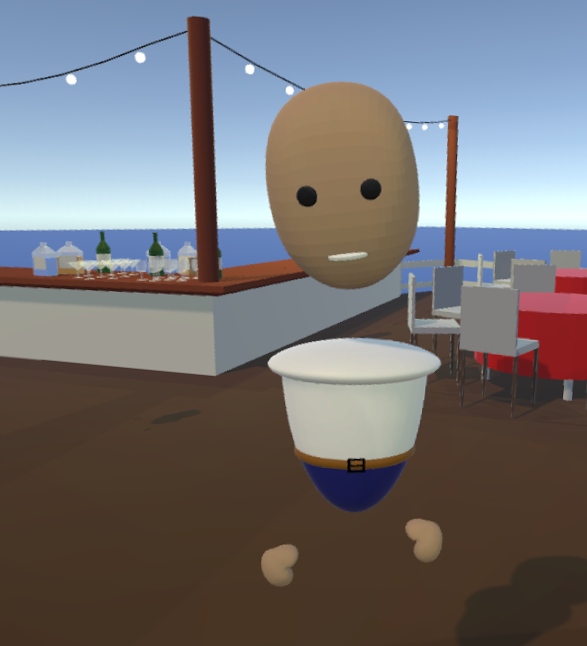
\includegraphics[width=.5\textwidth]{../graphics/environment_demo.png}
  \caption{Example view of the virtual environment, showing the cocktail party context and the avatar design.}
  \label{fig:system:environment_demo}
\end{figure}

\section{Identification Game Server}

The Identification Game Server utilize the built-in Unity3D network server to create an identification for each connected client, and notify the rest of the clients about new connections.
Based on this information clients create and manage avatars for all of the players in the virtual environment.
Usually, the Unity3D network server is also used to pass positioning, orientation, and other kinds of information between clients.
In this project, however, all of the data is passed between the clients through the Main Game Server.

\section{Main Game Server}

The main game server is used to pass information between the clients.
Each client repeatedly sends the player information to this server and get back information about the other players.
This information includes the positioning and orientation of the chest, head, and hands of the player.
It also includes the identification of who the player is looking at, whether or not the player is speaking (using sound level threshold), and whether or not the player is currently faking.

On the server, first, the player data is extracted from the HTTP request and stored in an in memory cache.
Then, information about the rest of the players is extracted from the cache.
For each of the non faking players, the information is passed to the client from the cache without modification.
Otherwise, the positioning and orientation are overridden by an automatic generated movement that are described thoroughly in section \ref{system:fake_behaviour_generator}.
Additionally, the player is flagged to be faking, and the identification of the current speaker is sent to the client.
This information is than used by the client to rotate the automated agent slowly towards the speaker.
I decided to implement this feature on the client side only for technical reasons:
Unity3D made it relatively straightforward to slowly rotate an object towards a specified direction, whereas on the server I would have to write this functionality from scratch.

The clients communicate with the server every 20 milliseconds, and interpolate the readings.
This fast communication is crucial for keeping the visual rendering smooth.
A faster communication rate found to overload the server.

The server is developed in \fnurl{Elixir}{https://elixir-lang.org/}.
Usually, when developing games in Unity3D the server is built with Unity3D as well.
The main reason I choose Elixir instead is my prior familiarity with it.
In addition, Elixir provides some nice benefits for this type of project, as it significantly simplifies the development of both web and concurrent programs.
Lastly, being a high level language with terse syntax and many high quality libraries accelerated the development process.

\section{Active Listening Server}\label{system:active_listening_server}

The Active Listening Server is responsible for predicting head nods.
It is based on the vast research in automatic backchannel behaviours prediction and uses speaker talking state (is speaking or silence) and gaze (is looking at listener or not).
Predicting listeners backchannel behaviours is usually done using either hand-crafted rule based systems, or more recently, data driven and machine learning (ML) approaches \citep{Morency2008}.
Due to the better performance of the later, and with the absence of openly available solution, I decided to develop an ML based backchannel predictor for the project.
Using more features, such as prosody \citep{Ward2000} or speaker gestures (TODO reference), could probably improve the model.
However, the simpler model described below was found to be accurate enough.

It is important to note that there is an expected difference in social behaviour between an addressee and a side-participant \citep{Clark1982}.
Although the addressee can fake active listening, in the context of the current research it is more common for side-participants to fake and wonder around, as they are not required to provide verbal response to the speaker.
However, there is much less literature about predicting side-participants active listening behaviours, and even less available resource for training a data-driven model.
With that in mind, I settled for predicting the addressee backchannels and applied them to both addressees and side-participants alike.

Training an ML model required a dataset of conversations with annotations for speaker talking state, gaze, and listener backchannels.
The ICT Rapport Dataset \citep{Gratch2007} contains 126 annotated interactions between a speaker and a listener, and is \fnurl{openly available online}{http://rapport.ict.usc.edu/}, making it ideal for training a backchannel predictor.
Many of the interactions, however, were not properly annotated.
Some of them doesn't contain all of the annotation files while other have blank columns for some of the features of interest.
After filtering out interactions with missing data the remaining 48 interactions had an average length of 138 seconds, ranging from 41 to 248 seconds.

To prepare the data for training I re-sampled the annotations every 100 milliseconds.
Then, to create samples representing a window moving in time I concatenate 30 samples (3 seconds) of the speaker talking state and gaze into one vector.
This vector, when fed into the ML model, should predict the listeners nodding of the last sample.
As a last step of preparation I split the dataset into 3 to 1 train and test portions.

I tried to train three different ML models.
First I attempted to train a Linear Support Vector Machine Classifier (LinearSVC) model using the open source software package Scikit-learn \citep{Pedregosa2011}.
Using the test portion of the dataset, the model precision (percentage of correct predictions) was high.
However, the recall (correct predictions out of correct predictions and misses) was very low.
In fact, the model learned to almost never predict a backchannel.
Visually comparing the predictions to the dataset reveals that the it failed to model the data correctly.
Second, I tried to train a Long Short-Term Memory (LSTM) deep neural network with the open source software package Keras \citep{Chollet2015}.
The results were similar to these of the LinearSVC model.
Lastly, I trained a K Nearest Neighbors classifier ($K = 5$) with Scikit-learn.
This time, it seems that the model manage to capture the nature of the data, as shown in figure \ref{fig:system:backchannel_predictions}.
Using the test portion of the dataset the accuracy was lower than before (0.77), but the recall was higher (0.83).

\begin{figure}
  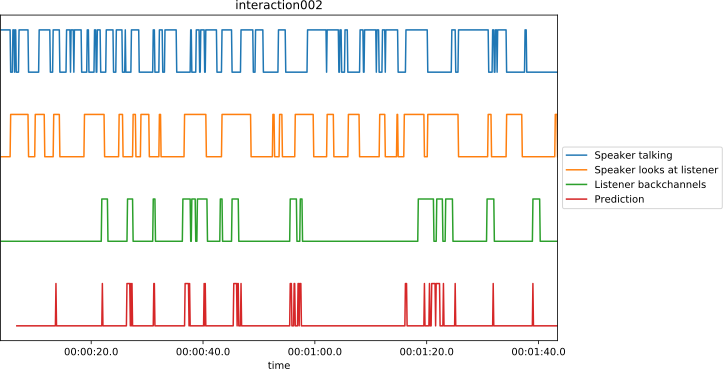
\includegraphics[width=\textwidth]{../graphics/backchannel_predictions.pdf}
  \caption{An example of one interaction between a speaker and a listener from the ICT Rapport dataset, with both actual and predicted listener backchannel behaviours. The lines indicate the state of the features and prediction with values of either 0 when the line is low, or 1 when the line is high.}
  \label{fig:system:backchannel_predictions}
\end{figure}

Choosing between the models didn't follow a properly nor systematic evaluation.
However, based on the performance on the test portion of the dataset and visual inspection the K Nearest Neighbors classifier seemed to performed well enough.
It also provided fast predictions, as necessary by real-time system like this one.

To make the backchannel predictions more robust to variations in the input data I implemented the variable threshold as suggested by \cite{Kok2012}.
The K Nearest Neighbors classifier can be used not only to predict a backchannel, as a binary value, but also to predict the probability of a backchannel.
This feature of the model is used, together with a variable threshold to provide predictions.
Initially, the threshold is set to 1, and is decreased over time by 10 percent per second.
When the predicted probability for a backchannel accedes the threshold, a backchannel is predicted and the threshold resets back to 1.

This model, with the variable threshold algorithm, is written in \fnurl{Python}{https://www.python.org/} and exposes an HTTP endpoint.
The code for this server is open sourced and \fnurl{available online}{https://github.com/Nagasaki45/backchannel}.
The Main Game Server repeatedly fetches all of the currently faking players from the server cache and sends them, together with information about the speaker talking state and gaze, to the Active Listening Server.
The returned predictions are stored back in the Main Game Server cache.

\section{Fake Behaviour Generator}\label{system:fake_behaviour_generator}

The Fake Behaviour Generator integrate the predicted head nods from the Active Listening Sever with a natural baseline recorded movement.
It is designed to provide a smooth and socially appropriate movement for the automated behaviour.
For each player, the position and orientation of the head and hands, relatively to the chest, is always recorded.
This data is kept in a 2 seconds buffer.
The decision to keep the last 2 seconds is arbitrary and found via trial and error.
It aimed to give a long enough recording to make the faked behaviour look natural, but in the same time not to include two old movements.
If the faker was involved in different type of activity few seconds ago, like speaking for example, it is better to discard these body movements as they are probably inappropriate in the new context.
When a participant start to fake active listening a playback of this buffer start from the last recorded sample and goes backwards until it reaches the beginning of the buffer, and then forwards again, repeatedly.
This ensure that there are no jumps in the playback of the recorded movement.

Lastly, the predicted head nods from the Active Listening Server are generating head nods animation that was created in Unity3D.
This animation is merged (position vectors are added together) with the rest of the faked behaviour.


\chapter{Evaluation}\label{evaluation}

The system described in the previous chapter suggests several interesting evaluation paths.
In the current study, I choose to follow the extensive research already done in the field of ECAs \citep{Nishimura2007, Bevacqua2008, Gratch2007, Huang2011, Lee2006, Poppe2013} and frame the evaluation in that context.
Whereas all of these studies assess interaction with an automated agent, in the current project the interaction is with an avatar that switches between human and automated control.
In addition, research in the field of ECAs doesn't usually explore multiparty social interactions.
These differences opens up ways to explore the properties of the transition between the two modes, and the effects of the social context.
More specifically, can state of the art ECA techniques (e.g. automated backchannel behaviours) seamlessly replace human controlled avatars?
If so, for how long can automated behaviour replace us without anyone noticing?
What underlying mechanisms are required to support such automated behaviour?
And more importantly, what are the limitations of such methods and what can they tell us about active listening behaviours?

This chapter presents a controlled experiment that was done to evaluate the automated active listening properties of the system, with emphasis on the properties of the transition into the automated behaviour.
Specifically, I assess the time it takes for participants to detect a faked behaviour, the detection accuracy, and how are these affected by familiarity between participants.
In addition, the participants strategies for detecting faked behaviour are analyzed and compared to their performance.
This information have the potential to explain what underlying mechanism more easily expose the automated behaviour.

\section{Methods}

% How to report participants gender / age: http://evc-cit.info/psych018/Reporting_Statistics.pdf
Participants were 6 males and 6 females aged 23 to 52 years (male: M = 33.67, SD = 9.71; female: M = 27, SD = 2.53)
Most of the participants were co-workers, friends, and classmates, that responded to my call for participants on mailing lists and private messages.
The participants were allocated to 4 groups of 3 participants each.
Due to missing a participant in one of the group a co-worker re-participated in the experiment.
Examination of the group and the participant data didn't show any unique or unexpected differences from the other groups so I decided not to discard the groups' data.

The participants were asked to cooperate in a hot air balloon task \citep{Howes2012} in the virtual environment:
They were presented with a scenario of an hot air balloon that is about to crash, unless one passenger will be sacrificed.
They had to come to an agreement, and choose between scarifying a 7 months pregnant woman, her husband, the balloon pilot, or their friend, a doctor that is about to find a cure for cancer.

They were also instructed that there are tokens hidden in the virtual environment that they need to find and collect, whilst still progressing towards their shared goal of the balloon task.
These tokens were presented only while faking, so to collect them they had to fake participation in the conversation.
Meanwhile, participants in the conversation could accuse whoever they think is faking active listening by looking at them and pressing a button on the hand controller.

A scoring mechanism was introduced to motivate the participants to use the faking behaviour:
Collecting a token gives 5 points.
A participant that correctly accuse another participant for faking stills one point from them.
However, if the accusation is incorrect, the accuser loses one point for the accused participant.

The experiment started by each participant filling a pre-experience questionnaire (see appendix \ref{appendix:questionnaire:pre}).
Then, the features and functions of the system were carefully explained using the instructions sheet found in appendix \ref{appendix:interface}.
Later, the participants entered the VR environment for 10 minutes familiarization session, after which the score of each participant for this session was revealed.
Participants were encouraged to ask questions about the system to make sure they fully understand how things work.
Then, the hot air balloon task was explained and the main experiment session was started.
I instructed the participants to get to an agreement in up to 15 minutes.
After the participants formed a consensus, the VR experience stopped.
Lastly, they filled a post-experience questionnaire (see appendix \ref{appendix:questionnaire:post}).

During the VR sessions the participants were divided into 3 network connected rooms, with one participant at each room.
They were video recorded and their view of the VR environment was captured.
The following events were logged by the system for further analysis:

\begin{itemize}
  \item Transitions to and from faked behaviours.
  \item Every time a participant started or stopped talking.
  \item Accusations for faking active listening.
  \item Collection of a token.
\end{itemize}

Note that this design, in general, contains only one condition: the group of participating interacting with each other in the VR environment.
Therefore, most of the results demonstrate the general characteristics of the system, without properly comparing them to any control condition.
Due to the absence of literature about this specific use of automated social behaviour, these results may provide a baseline for future research.

\section{Results}

Participants in the hot air balloon task reached a consensus by 10:41 to 14:49 minutes.
During that time, the ratio of correct accusations from all accusations made was 0.285.
Although this value is surprisingly low, it is above chance level, as the average ratio of time spent faking out of the entire session length is 0.22.
The ratio of faking behaviours that started and finished without any accusation was 0.787.
As shown in figure \ref{fig:analysis:hist_time_faking}, longer faking periods were easier to detect ($t(341) = -4.826$, $p < .001$).

\begin{figure}
  \centering
  \includegraphics[width=.6\textwidth]{../graphics/analysis_hist_time_faking.pdf}
  \caption{A histogram of the time, in seconds, of all faking behaviours. In blue are faking behaviours that started and finished without other participants accusing the faker. In orange are the faking behaviours that were detected: another participant correctly accused the faker. The figure demonstrates both the ratio between undetected and detected faking behaviours and the difference in time between undetected and detected faked behaviours.}
  \label{fig:analysis:hist_time_faking}
\end{figure}

A correlation was found between talking and faking behaviours.
More specifically, participants that talked a higher percentage of the experiment also faked active listening more time ($r(10) = 0.65$, $p < .05$) and for longer periods ($r(10) = 0.66$, $p < 0.05$).
This relationship, that is shown is the left panel of figures \ref{fig:analysis:correlation_talking_ratio_vs_faking_time} and \ref{fig:analysis:correlation_talking_ratio_vs_faking_ratio}, is mainly affected by one outlier.
Without the outlier there is no significant correlation, and the trend even change its general direction as shown in the right panel of figures \ref{fig:analysis:correlation_talking_ratio_vs_faking_time} and \ref{fig:analysis:correlation_talking_ratio_vs_faking_ratio}.
Therefore, the correlation between talking and faking behaviours might be understood as an unique strategy applied by a single participant.
Indeed, the written comments confirm that the participant tried to talk as much as possible while faking to distract the other participants:

\begin{figure}
  \centering
  \includegraphics[width=\textwidth]{../graphics/analysis_correlation_talking_ratio_vs_faking_time.pdf}
  \caption{Both panels show a scatter plot and a regression line of the participants' talking ratio (talking time out of the entire session) compared to the average faking time in seconds. In the left panel outliers, marked with orange, are included in the calculation. On the right panel outliers are excluded from the scatter plot, regression line, and statistics.}
  \label{fig:analysis:correlation_talking_ratio_vs_faking_time}
\end{figure}

\begin{figure}
  \centering
  \includegraphics[width=\textwidth]{../graphics/analysis_correlation_talking_ratio_vs_faking_ratio.pdf}
  \caption{Both panels show a scatter plot and a regression line of the participants' talking ratio (talking time out of the entire session) compared to the faking ratio (faking time out of the entire session). In the left panel outliers, marked with orange, are included in the calculation. On the right panel outliers are excluded from the scatter plot, regression line, and statistics.}
  \label{fig:analysis:correlation_talking_ratio_vs_faking_ratio}
\end{figure}

\begin{displayquote}
  \textit{
    FAKE IT TILL YOU MAKE IT.
    I was FAKING 50\% of experience, idea was to keep on talking load of things to make people engage while I do my thing.
    I was also getting more personal in my speech so people can believe that I'm there with them.
  }
\end{displayquote}

In addition, a negative correlation was found between average faking length (in seconds) of each participant and the ratio of faked behaviour they completed without being accused ($r(10) = -0.72$, $p < .01$).
This is inline with the previous results that shows that detected faking behaviours are usually longer.
Similarly to the correlations found between talking and faking behaviours, this correlation is also affected by the same outlier, as shown in figure \ref{fig:analysis:analysis_correlation_faking_time_vs_faking_undetected}.
In this case, again, removing the outlier makes the result insignificant.
However, the outlier keeps the general trend, suggesting that the failure to get significance without the outlier is not due to different underlying characteristics but due to reduced statistical power.
Therefore, I suspect that indeed, participant that choose longer periods of faking behaviour have less faked periods that complete without anyone noticing.

\begin{figure}
  \centering
  \includegraphics[width=\textwidth]{../graphics/analysis_correlation_faking_time_vs_faking_undetected.pdf}
  \caption{Both panels show a scatter plot and a regression line of the participants' average faking time in seconds compared to the ratio of undetected faking periods. In the left panel outliers, marked with orange, are included in the calculation. On the right panel outliers are excluded from the scatter plot, regression line, and statistics.}
  \label{fig:analysis:analysis_correlation_faking_time_vs_faking_undetected}
\end{figure}

Analysis of familiarity between the participants shows a positive correlation between familiarity and the percentage of correct accusations ($r_s = 0.19$, $p < .001$).
This can be viewed in figure \ref{fig:analysis:analysis_pointplot_familiarity_vs_correct}.

\begin{figure}
  \centering
  \includegraphics[width=.6\textwidth]{../graphics/analysis_pointplot_familiarity_vs_correct.pdf}
  \caption{The familiarity effect on the ratio of correct accusations. Familiarity between participants was measured on a 1 to 5 likert scale, and found to positively correlate with detection accuracy.}
  \label{fig:analysis:analysis_pointplot_familiarity_vs_correct}
\end{figure}

In addition to the quantitative data gathered during the VR experience, the post-experience questionnaires contain some interesting information about strategies for detecting faked behaviour.
Here, I will try to use this information and compare it with the participants statistics to see how the choice of strategies affected the participants performance in detecting faked behaviour.

Participant 7, for example, claimed the following:

\begin{displayquote}
  \textit{
    It wasn't as strategy to be honest I just could tell because the body language changed quite dramatically...
    For some reason it was quite obvious for me when participant 9 faked it.
    However, not so much when participant 8 did.
  }
\end{displayquote}

Let's see if this claim can be backed by the data collected by the system.
Participant 7 accused participant 8 five times, all of these accusations were incorrect.
Participant 9, on the other hand, was correctly accused 4 times (0.286 of the accusations) and incorrectly accused 10 times.
This ratio is almost the same as the already discussed 0.285 average ratio of correct accusations.
From this, we might assume that the claim is correct.
However, participant 8 faked only 0.056 of the time, while participant 9 faked 0.133 of the time, making the detection of participant 9 easier.
Overall, the claim must by at least partially true, as the participant did manage to accuse one better then the other.

Some participants pointed out more concrete strategies that helped them in detecting the faked behaviour.
Specifically, they claim to notice the underlying mechanisms behind the automated faked behaviour: looped recorded baseline, automated head nods, and rotating towards the speaker.
Let's see if participants that manage to understand how the system works, in one way or another, better detect faked behaviour.

Participants 12 and 14 indicated that they detected repetitive movement and used that as an indication for faking.

\begin{displayquote}
  \textit{Look for repetetive movement + create repetetive movement for myself.}

  \hfill
  --- Participant 12

  \textit{Watching for repetitive behaviours or behaviour that looked robotic.}

  \hfill
  --- Participant 14
\end{displayquote}

Using this strategy, 0.857 of the accusations made by participant 12 were correct.
As shown in figure \ref{fig:analysis:analysis_participant12_accusations_correct}, this value is significantly higher than the average 0.285 detection performance and is expected to exceed 99\% of the players ($z = 2.38$).
Participant 14, although performed above average with a ratio of 0.533 correct accusations, didn't reach significance ($z = 0.9$).

\begin{figure}
  \centering
  \includegraphics[width=.6\textwidth]{../graphics/analysis_participant12_accusations_correct.pdf}
  \caption{A normalized histogram and estimated distribution function of the ratio of correct accusations. Participant's 12 performance is significantly high on the upper tail of the distribution.}
  \label{fig:analysis:analysis_participant12_accusations_correct}
\end{figure}

Participants 5 and 8 looked for suspicious head nods to detect faked behaviour.

\begin{displayquote}
  \textit{Found head nods a good indicator even if they were fake.}

  \hfill
  --- Participant 5

  \textit{Noticing when the other participants just noded and didn't move their hands a lot}

  \hfill
  --- Participant 8
\end{displayquote}

Although automated head nods are indeed part of the underlying mechanisms of the automated faked behaviour, the detection performance of both participants was lower than average.
Therefore, and regardless of their claims, they probably didn't manage to differentiate correctly between real and faked behaviours based on head nods.
Participant 5, however, was \textit{\textquote{pressing `Accuse' loads}}.
This comment is backed by quantitative data: whereas the average participant made an accusation every 21 seconds, participant 5 made one every 5 seconds, which is considered higher than 99\% of the players ($z = 3.02$).
This is a result of partially misunderstanding of the scoring mechanisms.
So, there is a chance that the participant actually manage to detect the automated head nods, but that this is hidden behind the excessive accusations.
Overall, there is no clear evidence that any of the participants managed to improve their accusation performance based on faked head nods detection.

Lastly, participant 15 pointed out in the comments the last mechanisms to fake listening: looking at the speaker.
The participant detection performance was, however, lower than average, suggesting a failure to use this strategy to detect faked behaviour.

\begin{displayquote}
  \textit{Anyone facing me who was not talking was up for suspicion}

  \hfill
  --- Participant 15
\end{displayquote}

\section{Discussion}

The evaluation of the system provides some relatively surprising results.
The most prominent of them are the better than chance but nevertheless low accuracy in detecting faked active listening behaviours, and the high probability to start and finish faking without being noticed.
This suggests that the underlying mechanisms that automate the active listening behaviour usually manage to trick the players, and therefore are viable and useful for ECAs creation.
Furthermore, two of the underlying mechanisms are unique for the current system.
First, and as previously discussed, there is almost no research in ECAs in multiparty social contexts.
Always rotating towards the speaker was chosen as the simplest approximation for the automated agent attention.
As the analysis of the participants strategies shows, participants didn't manage to use this as a clue for detecting faked behaviour.
Therefore, I would argue that this mechanism supports the automated behaviour and without a more sophisticated attention mechanism it is essential for the faked behaviour credibility.
Second, no research in ECAs deals with transitioning between human and automated controlled behaviours.
The looped recorded baseline was mainly used to support this transition.
From the results, it seems that some of the participants managed to detect the loop and use that to differentiate between real and faked behaviour.
Therefore, improving the baseline behaviour might be the most important development path to achieve more reliable active listening behaviour.
Still, the generally low detection accuracy shows that the recorded baseline mechanism is not too obvious nor easy to detect.

Another surprising result is related to the backchannel behaviours implemented in this project.
I used only a small set of features and applied a single, simple, animation to the avatar.
Still, no participant managed to detect the faked behaviour by noticing the automated head nods.

Lastly, the results demonstrate clear positive correlation between participants familiarity and detection accuracy.
It might be interesting to explore further what cues helped familiar participants to improve their detection of faked behaviours.
I can only assume that participants manage to notice a decreased attention to the conversation indicated by verbal cues (e.g. ``er'' or ``ehh'' utterances).
The verbal cues from known participants might be more expected.
Similar reasoning might be applied to the body language with relation to the baseline recorded behaviour.
A future study might shed more light on this phenomena.


\chapter{General discussion}\label{general_discussion}


\chapter{Conclusions}\label{conclusions}

Use VR to investigate new ways of communication, and new social behaviours that are impossible in face to face conversation.

\section{Future work}

Many possible improvements to the idea and implementation.
Faking social behaviour is only one possibility.
Auto swap positioning.

The system developed in the current study suggests several interesting evaluation paths.
The first goes back to the comparison with traditional telephony.
Participants in phone conversation can always decide that it's time to end the call.
It is not the same as the decision to stop listening and start doing something else during the phone call.
Therefore, we may assume that when participants fake attention they do so with the intent to keep the conversation going.
This idea is transferable to the virtual environment developed in this study:
Participants can either leave the conversation by walking away, or start faking active listening and do whatever they want.
With that in mind, the system can be used to understand if faking active listening affect the level of conversations, and if so, how.
Extending this idea further, it might be interesting to check how the possibilities exposed by the system affect the overall group dynamics in the cocktail party context.

\begin{itemize}
  \item Require attention based on end-of-turn analysis instead of when someone is speaking with me.
  \item Jumping seamlessly between autopilots.
  \item Playback addressee in 4 seconds delay a la \cite{Bailenson2005}.
  \item Train an ML algorithm on VR data, not to predict head nods, but to generate hands and head transforms directly.
\end{itemize}


%%%%%%%%%%%%%%%%%%%%%%%%%%%%%%%%%%%%%%%%%%%%%%%%%%%%%%%%%%%%%%%%%%%%%%%%%%%%%%%%
%% Bibliography:
%%
\cleardoublepage
\phantomsection
\addcontentsline{toc}{chapter}{Bibliography}
\bibliographystyle{plainnat}
\bibliography{thesis}


\begin{appendices}


\chapter{Pre-experience questionnaire}\label{appendix:questionnaire:pre}

\begin{itemize}

\item Participant ID: $\rule{1cm}{0.1mm}$

\item What is your age? $\rule{1cm}{0.1mm}$

\item What is your gender?

\begin{itemize}
  \item Male
  \item Female
  \item Other $\rule{4cm}{0.1mm}$
  \item Prefer not to say
\end{itemize}

\item Have you experienced virtual reality with a head mounted display?

\begin{itemize}
  \item Never
  \item Once
  \item A few times
  \item Regularly
\end{itemize}

\item Have you experienced virtual reality with the HTC Vive?

\begin{itemize}
  \item Never
  \item Once
  \item A few times
  \item Regularly
\end{itemize}

\item Please rate how well you know each of the two other participants.

\begin{tabular}{c|C C C C C}
  & Do not know him/her at all & & & & Know him/her very well \\
  Participant ID $\rule{1cm}{0.1mm}$ & 1 & 2 & 3 & 4 & 5\\
  Participant ID $\rule{1cm}{0.1mm}$ & 1 & 2 & 3 & 4 & 5\\
\end{tabular}

\end{itemize}


\chapter{Post-experience questionnaire}\label{appendix:questionnaire:post}

\begin{itemize}

\item Participant ID: $\rule{1cm}{0.1mm}$

\item What were your strategies to maximize your score?

  \rule{\linewidth}{0.1mm}
  \rule{\linewidth}{0.1mm}
  \rule{\linewidth}{0.1mm}
  \rule{\linewidth}{0.1mm}
  \rule{\linewidth}{0.1mm}
  \rule{\linewidth}{0.1mm}

\item What were your strategies to detect that someone is faking attention?

  \rule{\linewidth}{0.1mm}
  \rule{\linewidth}{0.1mm}
  \rule{\linewidth}{0.1mm}
  \rule{\linewidth}{0.1mm}
  \rule{\linewidth}{0.1mm}
  \rule{\linewidth}{0.1mm}

\item Any other comment?

  \rule{\linewidth}{0.1mm}
  \rule{\linewidth}{0.1mm}
  \rule{\linewidth}{0.1mm}
  \rule{\linewidth}{0.1mm}
  \rule{\linewidth}{0.1mm}
  \rule{\linewidth}{0.1mm}

\end{itemize}


\chapter{Interface}\label{appendix:interface}

\begin{figure}[H]
  \includegraphics[width=\textwidth]{../graphics/interface_manual.pdf}
  \caption{Based on the HTC Vive controllers, the interface allows the players to teleport, fake active listening behaviours, and accuse other players for faking.}
  \label{fig:interface}
\end{figure}


\end{appendices}


\end{document}
